\documentclass [11pt]{article}
%Needed for fancy maths stuff
\usepackage{amsmath}
%Needed for Wits Style
\usepackage{url}
\usepackage{natbib} % Force natbib.sty to put citation labels in the reference list
\makeatletter
\renewcommand\NAT@biblabel[1]{\def\citeauthoryear##1##2{##1 ##2}[#1]\hfill}
\renewcommand\NAT@bibsetup[1]{%
  \setlength{\itemsep}{\bibsep}\setlength{\parsep}{\z@}}
\def\@lbibitem[#1]#2{%
  \if\relax\@extra@b@citeb\relax\else
    \@ifundefined{br@#2\@extra@b@citeb}{}{%
     \@namedef{br@#2}{\@nameuse{br@#2\@extra@b@citeb}}}\fi
   \@ifundefined{b@#2\@extra@b@citeb}{\def\NAT@num{}}{\NAT@parse{#2}}%
   \item[\hfil\hyper@natanchorstart{#2\@extra@b@citeb}\@biblabel{#1}%
    \hyper@natanchorend]%
    \NAT@ifcmd#1(@)(@)\@nil{#2}}
\makeatother


\bibpunct{[}{]}{;}{a}{}{}
%For figures
\usepackage{graphicx}
\usepackage{float}

\title{Building Bayesian Influence Ontologies\\Literature Review}
\author{Tamlin Love\\1438243}
\date{\today}

\usepackage[margin=1in]{geometry} %Margin size

\begin{document}
\maketitle
\section{Introduction}
In Section \ref{SimilarityMetrics}, we discuss a variety of classical approaches used to measure similarity. In Section \ref{BayesianNetworks}, we discuss the concept of a Bayesian Network. In Section \ref{ScoreBasedStructureLearning}, we discuss methods used to learn Bayesian network structures and evaluate them. In Section \ref{BayesianSimilarity}, we discuss the application of Bayesian Networks to measuring similarity.
\section{Similarity Metrics}\label{SimilarityMetrics}
\section{Bayesian Networks}\label{BayesianNetworks}
When considering a joint probability distribution across $n$ random variables, classical probability states that the number of parameters needed to represent the distribution grows exponentially in $n$ \citep{koller09}. Even in the simple case of binary variables, we would still need $2^n -1$ parameters to describe the distribution. This is clearly unfeasible for practical applications, in which the number of random variables can grow very large. 
\\
Bayesian networks, originally developed by \citet{pearl88}, present a way of reducing the number of parameters needed to represent a joint distribution. A Bayesian network is a directed acyclic graph (DAG) whose nodes represent random variables and whose edges represent influence of one variable on another. This structure can also be thought of as a representation of the conditional independencies between the random variables \citep{koller09}. Indeed, it is through the exploitation of these independency assumptions that a Bayesian network can more compactly represent a joint distribution.
\begin{figure}[H]\label{fig:sprinkler}
\centering
\caption{A famous example of a Bayesian network, showing how a complete representation of any random variable $X$ requires considering only those variables who are parents of $X$ in the graphical representation \citep{norvig94}.}
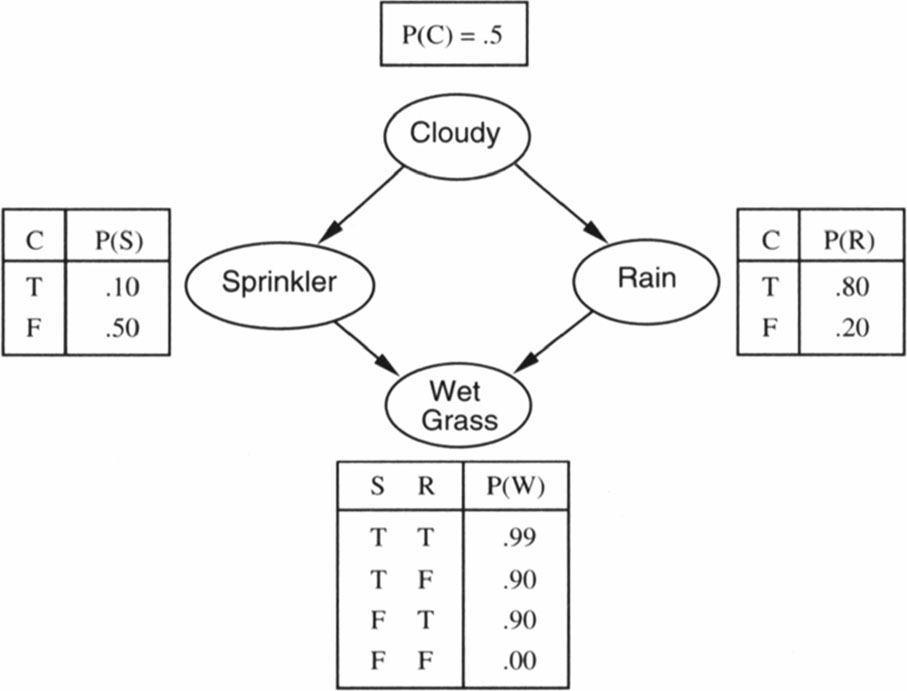
\includegraphics[width=8cm]{sprinkler.jpg}
\end{figure}
An important notion in Bayesian networks is that of d-separation, first presented by \citet{pearl86}, which is used to determine whether or not two sets of random variables are conditionally independent given another set. The set $\mathcal{I}(\mathcal{G})$ of conditional independencies in the graph $\mathcal{G}$ is used as the basis for an equivalence relation, I-equivalence, for which any two I-equivalent graphs represent the same independency assumptions \citep{verma91}.
\section{Score-Based Structure Learning}\label{ScoreBasedStructureLearning}
\section{Bayesian Similarity}\label{BayesianSimilarity}
\bibliographystyle{named-wits}
\bibliography{annot}
\end{document}